
\documentclass{IEEEtran}
% \textwidth 6.8in \addtolength{\oddsidemargin}{-1.1in}
% \textheight 10in
% \addtolength{\topmargin}{-0.5in}
% \setlength{\parindent}{0.0cm}
% \setlength{\parskip}{0.1cm}
% \topskip 0.0in

\usepackage{amsmath}
\usepackage{graphicx}
%date{August 08,2005}
%\date{\today}
\author{Yashasvi Jain(15UEC077), Tayba Wasim(15UCS150)} % The authors name
\title{IT WORKSHOP ENDSEM PROJECT } % The title of the document

\begin{document}
\maketitle


\begin{center}
\begin{LARGE}
\textbf{"How you look at the problem is pretty much how you'll see it"}\\
\end{LARGE}
\end{center}

\section{DIFFERENT ALGORITHMS FOR SORTING}
\label{sec:BUBBLE SORT}

\subsection{BUBBLE SORT}
Bubble Sort works by repeatedly stepping through lists that
need to be sorted , comparing each pair of adjacent items
and swapping them if they are in the wrong order.


\subsection{INSERTION SORT}

Insertion Sort inserts each item into its proper place in the
final list.The simplest implementation of this requires two
list structures- the source list and the list into which the
sorted items are inserted.


\subsection{MERGE SORT}
Merge Sort splits the list to be sorted into two equal halves
and places them in separate arays.Each array is recursively
sorted and then merged back together to get the final sorted list.

\subsection{QUICK SORT}
Quick Sort is an in-place , divide and conquer, massively
recursvie sort. It’s essentially in-place version of the merge
sort.
\subsection{SELECTION SORT}
Selection Sort is an in-place comparison sort.It is inefficient
on large lists and generally performs worse than similar
insertion sort.
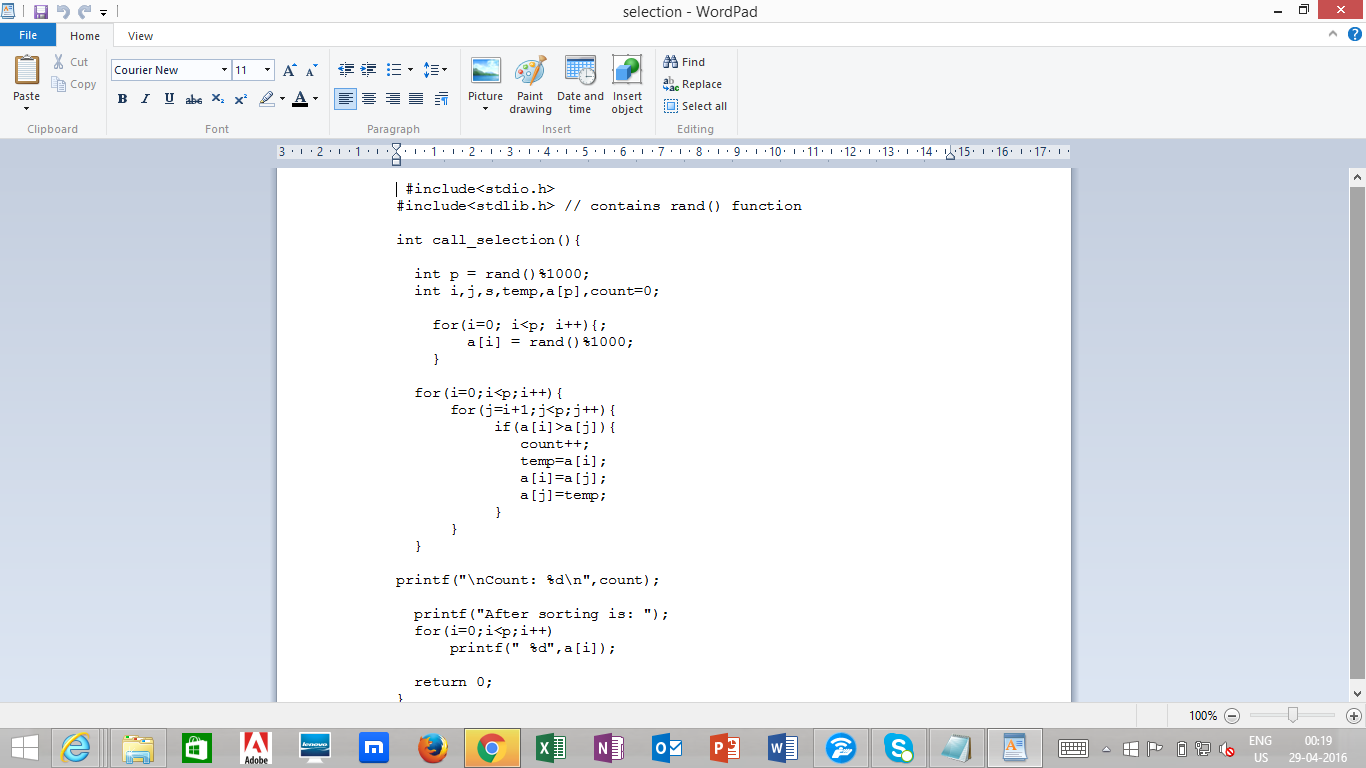
\includegraphics[height=3in,width=3in]{../Desktop/Screenshot (2)(1).png}
\section{WHICH SORTING ALGORITHM IS THE BEST?}
\subsection{Number of Comparison(in worst case) Vs number of Elements(n is the number of elementsin the array}

\begin{tabular}{|c|c|}
\\
\hline 
Sorting Algorithm & Number of Comparisons\\
\hline 
Bubble Sort & O($n^2$)\\
\hline 
Insertion Sort & O($n^2$)\\
\hline 
Merge Sort & O($nlogn$)\\
\hline 
Quick Sort & O($n^2$)\\
\hline 
Selection Sort & O($n^2$)\\
\hline 
\end{tabular} 
\section{Conclusion}
If the data set is small, it is semmed that bubble sort is the best sort since it is faster while in case of large data set Merge sort is the best sort since it does not matter how much the memory it takes as it divides array into two halves.


\end{document}
 
 
\grid
